\documentclass{article}

\usepackage[utf8]{inputenc}
\usepackage[margin=1in]{geometry}
\usepackage[colorlinks=true, pdfborder={0 0 0}]{hyperref} 
\usepackage{microtype}
\usepackage{amsfonts}
\usepackage{amssymb}
\usepackage{graphicx}
\usepackage{subfig}
\usepackage{float}
\usepackage{siunitx}
\usepackage{listings}
\setcounter{topnumber}{8}
\setcounter{bottomnumber}{8}
\setcounter{totalnumber}{8}
\usepackage{arydshln}
\usepackage[framemethod=tikz]{mdframed}
\usepackage{minted}
\usepackage{empheq}
\usepackage{nicematrix}
\usepackage{titlesec}

\usepackage[sorting=nty]{biblatex}
\addbibresource{sources.bib}

\setlength{\parindent}{0cm}
\setlength{\leftskip}{0cm}

\usepackage{amsmath}
% For annet format på formler:
% \usepackage[fleqn]{amsmath}
% \setlength{\mathindent}{0cm}

\lstset{
  language=Python,
  basicstyle=\footnotesize\ttfamily,
  %keywordstyle=\color{blue},
  %commentstyle=\color{green},
  %stringstyle=\color{red},
  numbers=left,
  numberstyle=\tiny,
  numbersep=5pt,
  breaklines=true,
  showstringspaces=false,
  xleftmargin=.25in,
  xrightmargin=.25in
}

\definecolor{barcolor}{rgb}{0.9,0.9,0.9}
\renewenvironment{leftbar}[1][\hsize]{
    \def\FrameCommand{{\color{barcolor}\vrule width 2pt \hspace{10pt}}}
    \MakeFramed{\hsize#1 \advance\hsize-\width \FrameRestore}
}{\endMakeFramed}

\titleformat{name=\section,numberless}[block]
  {\normalfont\Large\bfseries}
  {\llap{\rule[0ex]{0.6em}{0.6em}\hspace{1.8em}}}{0em}{\titlerule\\[.8ex]}{}

\renewcommand\thefootnote{\textcolor{black}{\arabic{footnote}}}
\renewcommand{\footnoterule}{}

\setlength{\parskip}{0.15cm}

\begin{document}

\begin{center}
    \textbf{\LARGE Reinforcement learning}

    %\rule{4cm}{1pt}
    \vspace{0.2cm}
    
    2024

\end{center}

\section*{Motivation}

Reinforcement learning is, in simple terms, a method where an artificial neural network (hereafter Agent) is placed in an environment with instant or delayed feedback in regard to the environment. This feedback is what makes the Agent able to learn. An example of this would be a chess-playing Agent whose input is an image of the board and output its next move in response to the input. The feedback the Agent receives could then be piece captures, position evaluations, etc. Within reinforcement learning the input to the Agent is usually referred to as the "state", and the output as the "action".

An Agent usually starts its learning process from scratch, and has to figure out which actions lead to positive feedback. Therefore, many iterations are needed to learn weights corresponding to mastering the task at hand. This process may in some cases be challenging, especially if the feedback is significantly delayed - which makes it hard for the Agent to determine which of the actions led to the positive feedback.

OpenAIs work on mastering Minecraft had a goal for their Agent to obtain diamond tools, which "usually takes proficient humans over 20 minutes (24,000 actions)" (\textit{i.e.} extremely delayed feedback), and achieved this through sequential rewards \cite{Minecraft}. Likewise, if the feedback for a chess-Agent is the end result of a game, it is hard for the Agent to distinguish between good and bad moves throughout the game. Therefore, like OpenAIs solution, step-wise feedback (\textit{e.g.} piece captures and position evaluations in chess) is a good strategy for speeding up the learning process.

\section*{Cart-pole environment}

\begin{minipage}{.5\textwidth}
  To gain a basic understanding of how reinforcement learning works one can experiment with a "simple" problem. The cart-pole problem being such, is an environment where an Agent has to balance a pole on top of a cart by moving it either to the left or the right — based on the current state of the environment.
\end{minipage}%
\begin{minipage}{.5\textwidth}
  \centering
  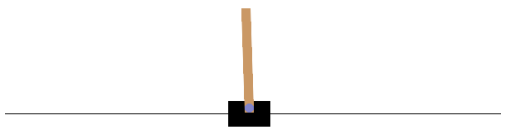
\includegraphics[width=.8\linewidth]{images/cart-pole.png}
\end{minipage}

\vspace{0.2cm}

The cart-pole environment is a part of the \textit{Gymnasium} package in python. This package contains a number of different virtual environments which can be imported and used to train and validate ones own reinforcement Agents. \cite{Gymnasium} \cite{Cart-pole} The environment is created and initialized by the following lines of python code:

\vspace{0.2cm}

\begin{lstlisting}
    import gymnasium as gym
    
    environment = gym.make('CartPole-v1', render_mode="rgb_array")
    observation, info = environment.reset()
\end{lstlisting}

The Agent controls the cart movement, \textit{i.e.}, by pushing it one way or another. The action is therefore binary, being $0$ or $1$ for respectively pushing the cart to the left or the right. By being able to observe the current state of the cart position, cart velocity, pole angle and pole angular velocity, the Agent has to choose an appropriate action. A reward is given for every time-step until the pole is no longer standing. The termination (or truncation) is determined by whether the pole angle is greater than $\pm 12 ^\circ$, the cart position is more than $\pm 2.4$ (too far away), or the episode length is greater than $500$ time-steps.

\subsection*{The Agent}
\begin{leftbar}
    The Agent is a neural network which takes the current observed state as input and returns the chosen action based on this.

    Where Barto, Sutton and Anderson used "two types of neuronlike adaptive elements [...] an \textit{associative search element} (ASE) and the other an \textit{adaptive critic element} (ACE)" \cite{Neuronlike}, we intend to first experiment with a single Agent.

    A simple Agent can be created using \textit{torch} as seen below. Here, an arbitrary $64$ units are chosen for the hidden layer.

    \begin{lstlisting}
    import torch
    import torch.nn as nn
    
    class Agent(nn.Module):
        def __init__(self):
            super(Agent, self).__init__()
            
            self.layer_in = nn.Linear(4, 64)
            self.layer_hidden = nn.Linear(64, 64)
            self.layer_out = nn.Linear(64, 1)
            
        def forward(self, x):
            _output = torch.tanh(self.layer_in(x))
            _output = torch.tanh(self.layer_hidden(_output))
            output = self.layer_out(_output)
            
            return output
    \end{lstlisting}

    Note that this is an extremely simplified architecture, and that multiple hidden layers of variable units may be added, different activation functions used, etc.

\end{leftbar}
\subsection*{Policy-based learning}
\begin{leftbar}
    h
\end{leftbar}
\subsection*{Value-based learning}
\begin{leftbar}
    h
\end{leftbar}
\subsection*{Training}
\begin{leftbar}
    When training the Agent, one has to determine how to calculate the loss. This can either be a generalized or tailored approach, depending on the use-case of the Agent. In the letter by Mnih \textit{et.al.} they chose an approach that generalized well across tasks; "a single algorithm that would be able to develop a wide range of competencies on a varied range of challenging tasks" \cite{Human-level}. 
    
    However, in the case of the cart-pole problem, a simpler architecture and loss function is preferred. If the Agent is supposed to generalize well across tasks, a relatively large architecture is needed in order to handle all cases. This, in turn, leads to a significantly longer training-time.
\end{leftbar}

%{\centering 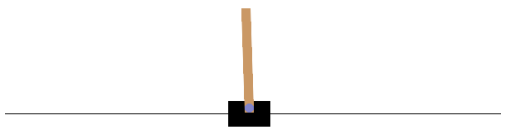
\includegraphics[width=8cm]{images/cart-pole.png} \par}

\newpage
\printbibliography

\end{document}
